\chapter{Introdução}

O desenvolvimento de software passou, e de certa forma ainda passa, por uma fase conhecida como \emph{crise do software}, termo utilizado pela primeira vez por \citeonline{HumbleProgrammer}. A Engenharia de Software surgiu \cite{NaurRandell} numa tentativa de contornar esta crise. No entanto, ela foi baseada em algumas considerações equivocadas, que serão abordadas posteriormente, fazendo com que falhasse na sua tentativa de contornar tal crise.

Com o passar dos anos, o mercado demanda e espera software inovadores e de alta qualidade, que sejam adequados a suas necessidades $-$ e o mais rápido possível \cite{TheBusinessOfInnovation}. Como isso não foi praticável através do Engenharia de Software tradicional, buscou-se uma abordagem alternativa.

O desenvolvimento ágil de software, que neste ano de 2012 completa 11 anos, foi elaborado \cite{AgileManifesto} para resolver esta crise que a Engenharia de Software tradicional não conseguiu, focando nas pessoas ao invés do processo e abraçando as mudanças ao invés de evitá-las. De acordo com \citeonline{PMNetworkFailureDrop}, o \textit{Chaos Manifesto 2011}\footnote{O \textit{Chaos Manifesto} é uma pesquisa bienal realizada pelo \textit{The Standish Group} e teve início em 1994. As pesquisas publicadas em um ano representam os dados do ano anterior.} mostra que os resultados de 2010 representam, desde sua primeira edição, a maior taxa de sucesso nos projetos de desenvolvimento de software, que aumentou de 32\% em 2008 para 37\% em 2010. Segundo \citeonline{ResumoChaosReport}, o \textit{The Standish Group} conclui que uma das principais razões para o aumento da taxa de sucesso foi a utilização das metodologias ágeis, que cresce a uma taxa de 22\% CAGR\footnote{\href{http://en.wikipedia.org/wiki/Compound_annual_growth_rate} {Compound annual growth rate}} e hoje são adotados em 9\% de todos os projetos de TI em andamento e em 29\% dos novos projetos.

Como o desenvolvimento ágil é relativamente novo, diversos métodos e técnicas vem sendo desenvolvidos tendo como base os princípios e valores ágeis \cite{BDDRodrigo}, principalmente relacionadas ao teste de software. Sendo técnicas emergentes, ainda são pouco discutidas no meio acadêmico, este trabalho pretende contribuir com esta discussão e, de certa forma, com a introdução de técnicas vindas do mercado na academia.


\section{Justificativas e objetivos}

Existe uma enorme escassez de trabalhos acadêmicos no que se refere a técnicas emergentes de testes de software, como notado também por \citeonline{BDDSolis}, que em 2011 foram os primeiros a ter um artigo publicado sobre BDD, pela \textit{IEEE Computer Society}.

Sendo assim, o objetivo do presente trabalho é contribuir com a introdução de técnicas e discussões surgidas no mercado para a academia, além agregar conhecimentos, ora dispersos e difusos, sobre as diferentes abordagens, possibilidades e pontos em aberto no emprego de tais técnicas.

As técnicas que serão abordadas neste trabalho tem seu conceito definido no mercado e evoluem através da evolução das ferramentas que os implementam. O fluxo de evolução é o seguinte: cria-se um conceito e uma ferramenta que o implemente. Com base na utilização e observação desta ferramenta, há uma percepção de novas necessidades, fazendo que novas ferramentas sejam criadas e que os conceitos evoluam. Desta forma, a informação e os diferentes conceitos estão dispersos, pois nunca foram sistematizados, ficando em uma espécie de ``inteligência coletiva"\ da comunidade $-$ comunidade esta que é ainda pequena, sendo um tipo de ``elite"\ dos desenvolvedores, que são os que de fato utilizam estas técnicas atualmente.

Além disso, como a literatura tradicional tem dificuldades em relacionar a teoria e prática, quase nunca utilizando exemplos em código, torna-se penosa a tentativa do leitor compreender de fato e aplicar os conceitos abordados.

Dessa forma, como o presente trabalho está no contexto dos métodos ágeis, e nestes as partes conceitual e prática formam um todo inseparável, para toda técnica abordada serão utilizados exemplos mostrando código de um projeto real.

\section{Metodologia}

Será feita uma explanação sobre cada técnica e uma discussão comparando as diferentes abordagens, possibilidades e pontos em aberto no emprego de cada técnica.

Como base para a discussão, será utilizado o kanban-roots\footnote{\url{http://github.com/hugomaiavieira/kanban-roots}}, que está sendo desenvolvido em conjunto com o presente trabalho.

O kanban-roots é um kanban\footnote{O termo tem origem no sistema Toyota de produção, onde kanban é a maneira como é coordenado o fluxo de peças na cadeia de suprimentos  \cite{AMaquinaQueMudouOMundo}. No contexto do presente trabalho, kanban é um quadro para visualização do fluxo de trabalho (tarefas) em um projeto.} online para auxiliar a organização e acompanhamento das tarefas em um projeto, sendo especialmente interessante para projetos \textit{opensouce} ou, de modo geral, para projetos com equipes geograficamente distribuídas.  O kanban-roots já está em produção e vem sendo testado e utilizado com sucesso por algumas pessoas e empresas, não só do Brasil, mas também da França, Lituânia, Polônia, Africa do Sul, Rússia, Inglaterra, China, Finlândia, Peru, Estados Unidos, entre outros.

Na figura \ref{img:tela_kaban_roots} pode ser visto um \textit{print} da tela do kanban de um projeto no kanban-roots.

\begin{figure}[h]
  \center
  \caption{Tela do kanban de um projeto no kanban-roots}
  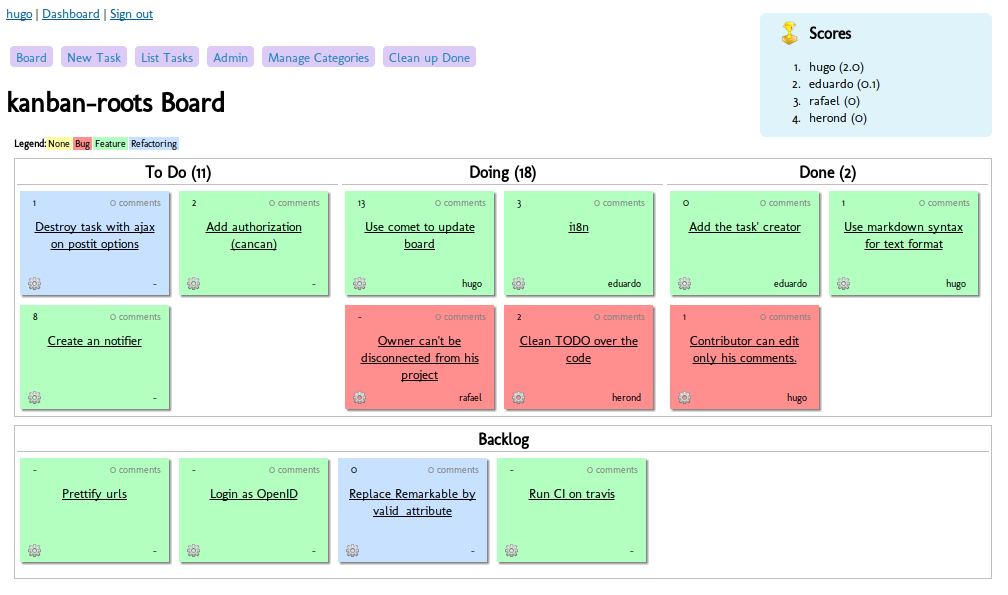
\includegraphics[scale=0.45]{images/kanban-roots}
  \label{img:tela_kaban_roots}
\end{figure}

Todos os trechos de código apresentados neste trabalho são trechos retirados do kanban-roots. A primeira linha de cada trecho sempre é um comentário informando o nome do arquivo original.

\section{Ferramentas utilizadas}

Para o desenvolvimento do kanban-roots foram utilizadas diversas ferramentas, sendo importante citar em que contexto e momento cada uma delas é utilizada.

Como base para o desenvolvimento, foi utilizado o \textit{framework web} Ruby On Rails\footnote{\url{http://rubyonrails.org}}. Para os testes de unidade apresentados na Seção \ref{sec:tdd} foi utilizado o Test::Unit\footnote{\url{http://test-unit.rubyforge.org/}}. Já na Seção \ref{sec:bdd} é utilizado o Rspec\footnote{\url{http://rspec.info/}} para testes unitários, testes de aceitação e dublês de teste. Ainda na Seção \ref{sec:bdd} também foi utilizado o Cucumber\footnote{\url{http://cukes.info/}} para testes de aceitação. Além dessas ferramentas, também foi utilizado o FactoryGirl\footnote{\url{https://github.com/thoughtbot/factory_girl}} para \textit{fixtures replacement} em todos os momentos em que se fez necessário.

\section{Trabalho relacionados} % (fold)
\label{sec:trabalho_relacionados}

Existem pouquíssimos trabalhos acadêmicos relacionados às técnicas abordadas no presente trabalho, e todos eles abordam o tema apenas conceitualmente, deixando uma lacuna de uma parte prática para complementar e favorecer o entendimento.

\citeonline{BDDSolis} apresentam algumas das principais características do \textit{Behaviour-Driven Development} (BDD), tendo como base a pequena literatura relevante e as ferramentas existentes para a utilização da técnica.

Sobre \textit{Test-Driven Development} (TDD), praticamente são apenas encontrados estudos empíricos, com estudos de caso na academia e na indústria, que discutem a efetividade do uso do TDD. Na Seção \ref{sub:a_efetividade_do_tdd} será feita uma análise destes estudos.

% section trabalho_relacionados (end)